%---------------------------------------------------
% Nombre: capitulo1.tex  
% 
% Texto del capitulo 1
%---------------------------------------------------

\chapter{Modelado}

En esta primera pr�ctica se pide realizar un modelado sencillo de un objeto, de manera que el modelo se asimile lo m�ximo posible al objeto real del que proviene. En la secci�n \ref{modelo} veremos por tanto el objeto del que parte el proceso de modelado que veremos explicado finalmente en la secci�n \ref{modelo2}.


\section{Modelo elegido}
\label{modelo}


El modelo escogido para esta primera pr�ctica podemos verlo en la figura \ref{img_1}. En el podemos ver el \textit{sable l�ser} de Luke Skywalker en la la pel�cula \textit{Star Wars}. Es un modelo aparentemente sencillo y que nos permite probar las primitivas b�sicas de blender para una primera aproximaci�n al software. Por otro lado, contiene detalles y que hacen del desarrollo del modelo con este objeto una pr�ctica muy interesante de cara a aprender Blender. 

\begin{figure}[h]
	\centering
		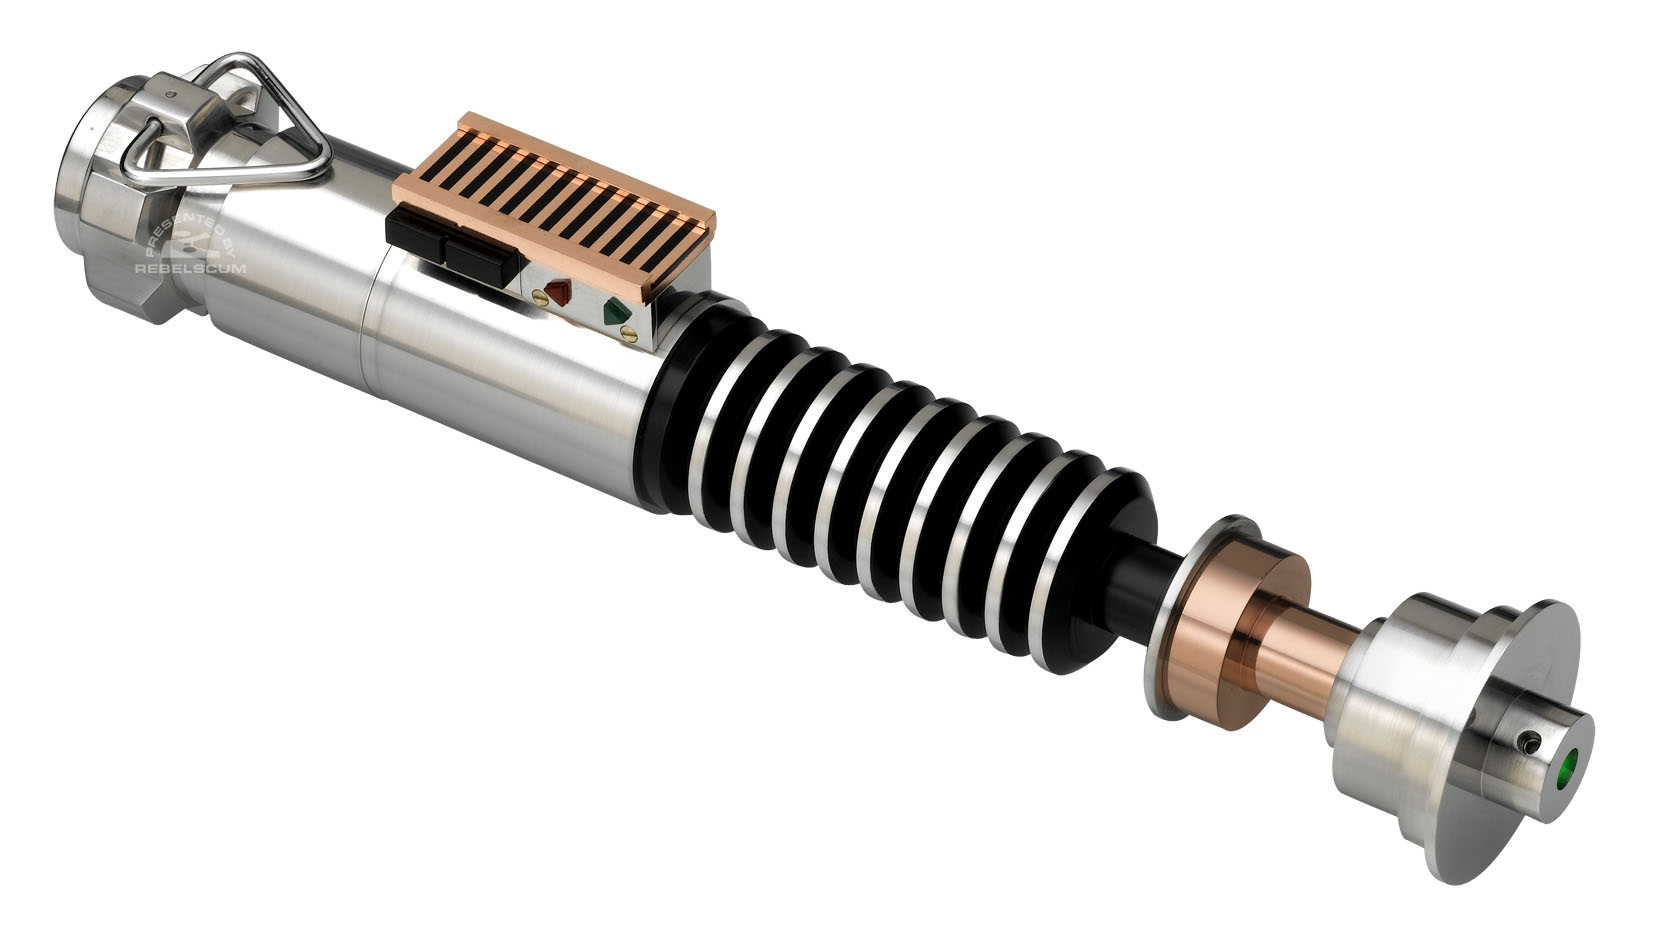
\includegraphics[scale=0.25]{./Capitulo1/Imagenes/sable.jpg}
		\caption{Sable laser de Luke en Star Wars VI.}
	\label{img_1}
\end{figure} 

Por otro lado, hay multitud de bibliograf�a y tutoriales  \cite{1} \cite{2} \cite{3} dedicados al desarrollo de un modelo similar por lo que de cara a problemas o dudas al respecto la comunidad es extensa al respecto. 

\section{Proceso de modelado}
\label{modelo2}

En esta secci�n veremos los pasos seguidos para modelar el sable l�ser. Somos conscientes de que al ser un objeto circular, podr�a haberse usado el modelado por revoluci�n pero dado que el objetivo de la pr�ctica era aprender las primitivas b�sicas del modelado en blender nos hemos centrado en modelar manualmente el objeto. 

Para comenzar a modelar el sable comenzamos con un cilindro en visi�n ortho y desde arriba. Al cilindro le quitaremos el relleno al momento de crearlo y le aplicaremos una rotacion de 90� sobre el eje X. El resultado podemos verlo en la figura \ref{2}.

\begin{figure}[h]
	\centering
		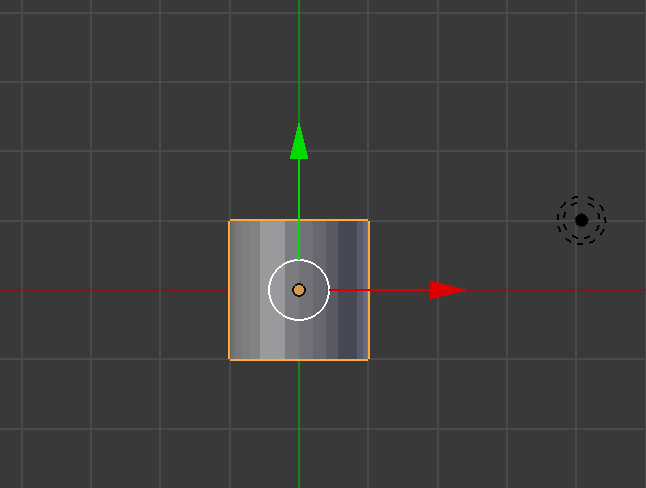
\includegraphics[scale=0.5]{./Capitulo1/Imagenes/2.png}
		\caption{Primer paso del modelado. Cilindro}
	\label{2}
\end{figure} 

Tras esto llega el momento de comenzar a modelar por lo cual haciendo uso de los comandos de escalado (shortcut S) y estrusi�n (shortcut E) iremos dando forma alargada como podemos ver en la figura \ref{3}. Sobre esta figura hemos aplicado cortes (ctrl+R), los cuales generan caras nuevas, para estilizar ciertos puntos en pasos posteriores. En la figura \ref{3}, podemos ver como mediante estos cortes hemos creado una regi�n que albergar� los discos de nuestro sable laser, para la cual realizaremos 18 cortes nuevamente, y que por medio de selecci�n de anillos, (sifht+alt+select) seleccionaremos y reduciremos su tama�o como podemos ver en las figuras \ref{4} y \ref{5}.

\begin{figure}[h]
	\centering
		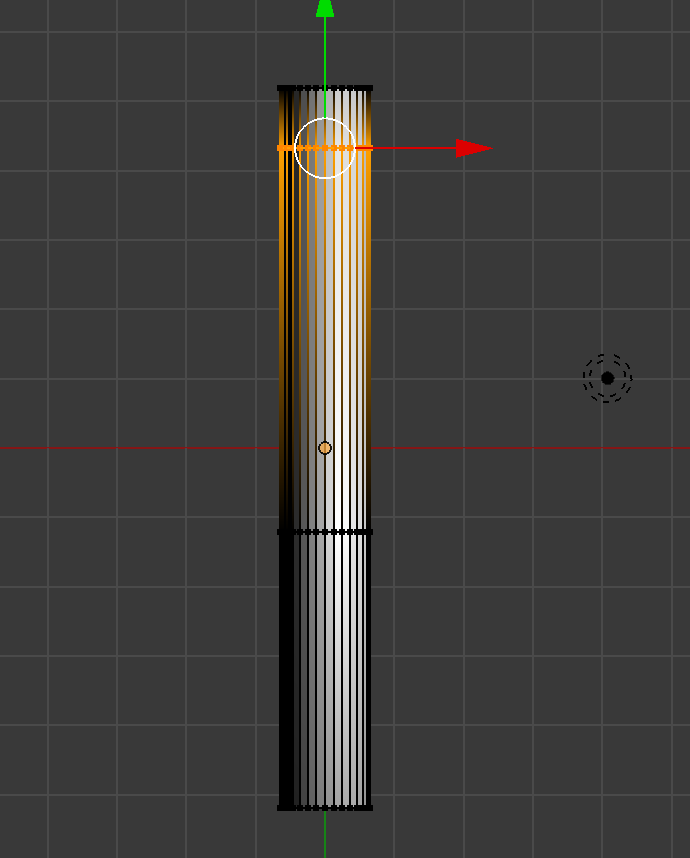
\includegraphics[scale=0.4]{./Capitulo1/Imagenes/3.png}
		\caption{Segundo paso del modelado. Cilindro alargado con cortes.}
	\label{3}
\end{figure} 


\begin{figure}[h]
	\centering
		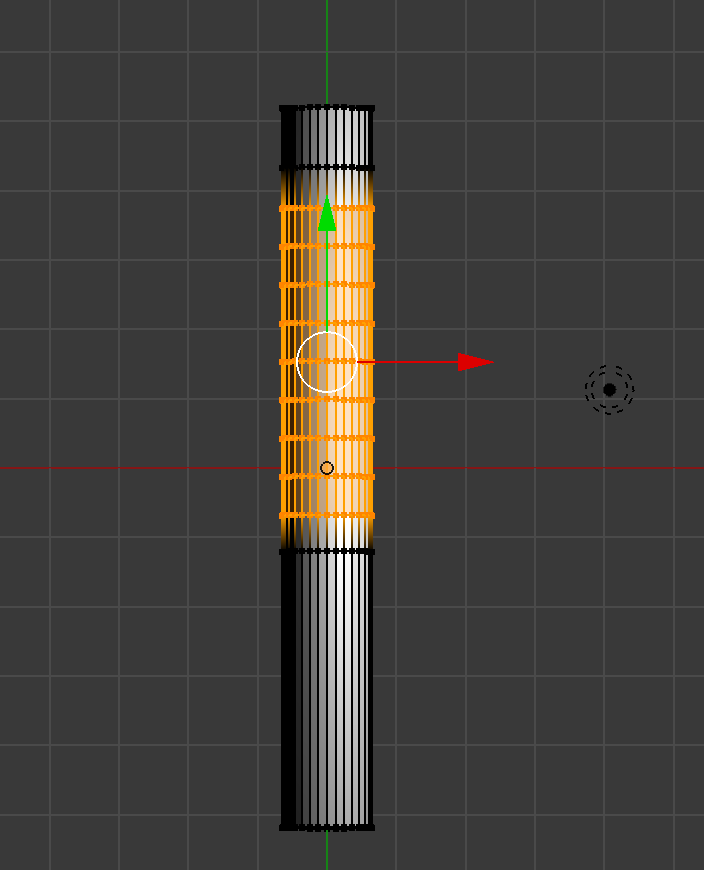
\includegraphics[scale=0.4]{./Capitulo1/Imagenes/4.png}
		\caption{Cortes para los discos.}
	\label{4}
\end{figure} 

\begin{figure}
	\centering
		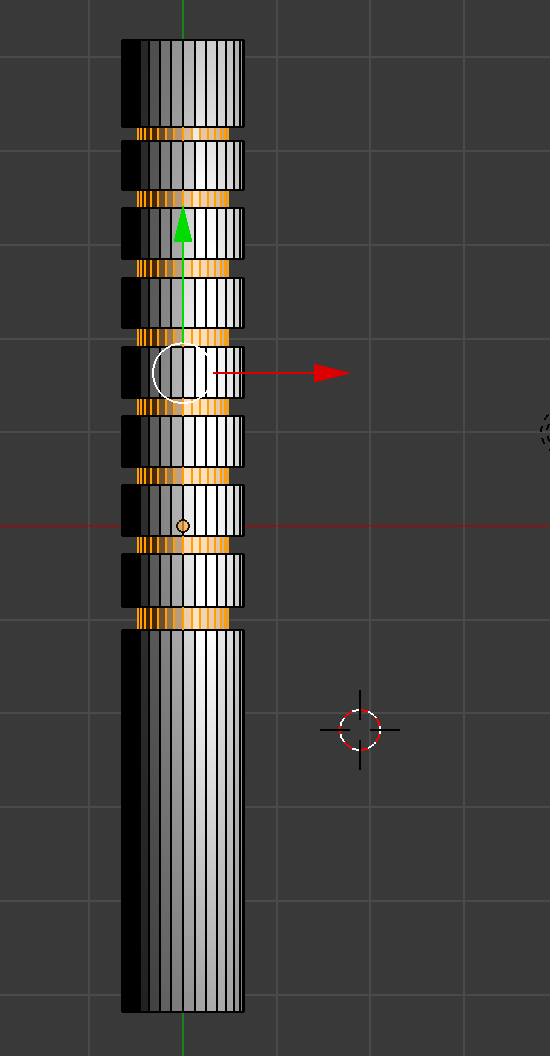
\includegraphics[scale=0.4]{./Capitulo1/Imagenes/5.png}
		\caption{Reducci�n del tama�o de los discos.}
	\label{5}
\end{figure} 


El siguiente paso pasa por modelar la punta del l�ser. Pasaremos a selecci�n por v�rtices y seleccionaremos el anillo de v�rtices de la punta. Tras esto usando las primitivas de escalado y estrusi�n, de nuevo vamos generando la forma deseada eligiendo siempre el eje apropiado para aplicar la transformaci�n y evitar que podamos torcer el puntero y por ende el objeto. Una imagen del proceso podemos verla en \ref{6}.

\begin{figure}
	\centering
		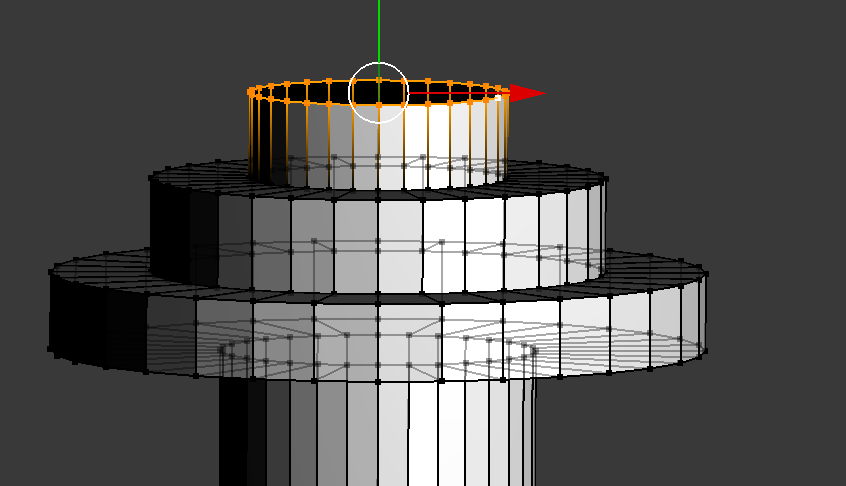
\includegraphics[scale=0.4]{./Capitulo1/Imagenes/6.png}
		\caption{Punta del laser.}
	\label{6}
\end{figure} 

Para realizar el rallo l�ser, una vez creada la punta, por medio de estrusi�n, llevamos la ultima fila de v�rtices hacia el centro del sable para estilizar. Tras ello, copiamos este ultimo anillo de v�rtices que como hemos dicho hemos llevado al interior del arma, y por ultimo hacemos un escalado de la misma en el eje Y. El siguiente paso ser� cerrar el sable, para ello seleccionamos el ultimo anillo de v�rtices del mismo por la parte de abajo, pulsamos E luego S y 0 para cerrar en el origen, el resultado podemos verlo en la figura \ref{7}

\begin{figure}
	\centering
		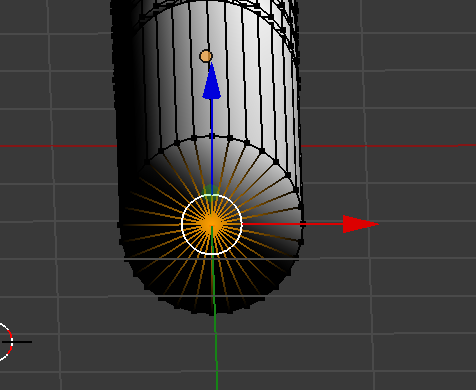
\includegraphics[scale=0.6]{./Capitulo1/Imagenes/12.png}
		\caption{Tapas del arma.}
	\label{7}
\end{figure} 

Una vez hecho esto solo nos quedar� adornar el sable l�ser. Para ello hacemos cortes en la base para generar las caras que usaremos para dar relieve a ciertos puntos. El resultado de esta partici�n podemos verlo en la imagen \ref{8}. 


\begin{figure}
	\centering
		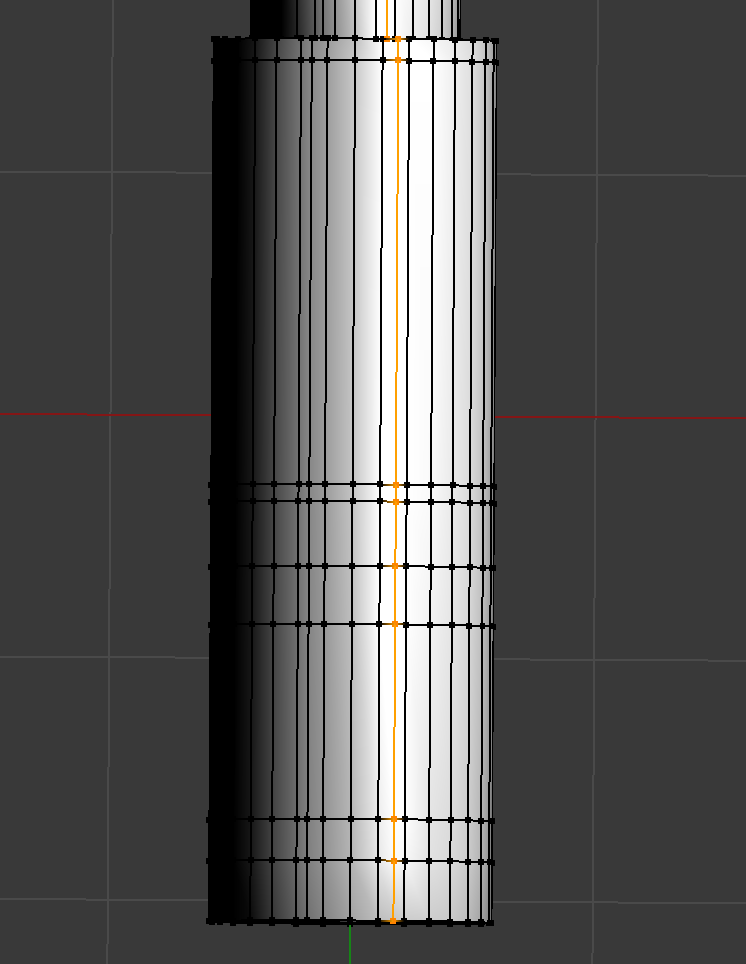
\includegraphics[scale=0.4]{./Capitulo1/Imagenes/8.png}
		\caption{Caras para adornar.}
	\label{8}
\end{figure} 

Por �ltimo solo nos queda adornar el modelo. En un primer paso  aumentamos el tama�o de ciertos elementos dando relieve para que se asimile m�s a la realidad tal y como podemos ver en las figuras \ref{9} \ref{10} \ref{11} y \ref{12}.

\begin{figure}
	\centering
		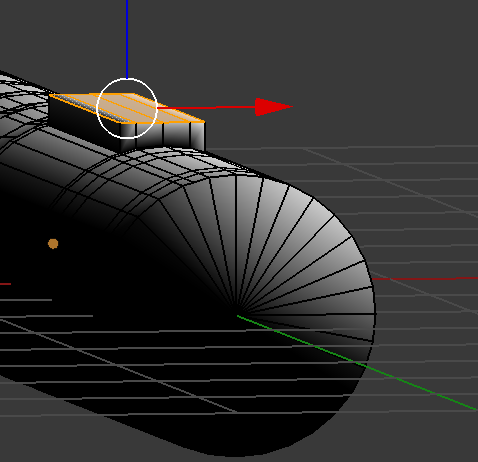
\includegraphics[scale=0.6]{./Capitulo1/Imagenes/9.png}
		\caption{Botones sable 1.}
	\label{9}
\end{figure} 

\begin{figure}
	\centering
		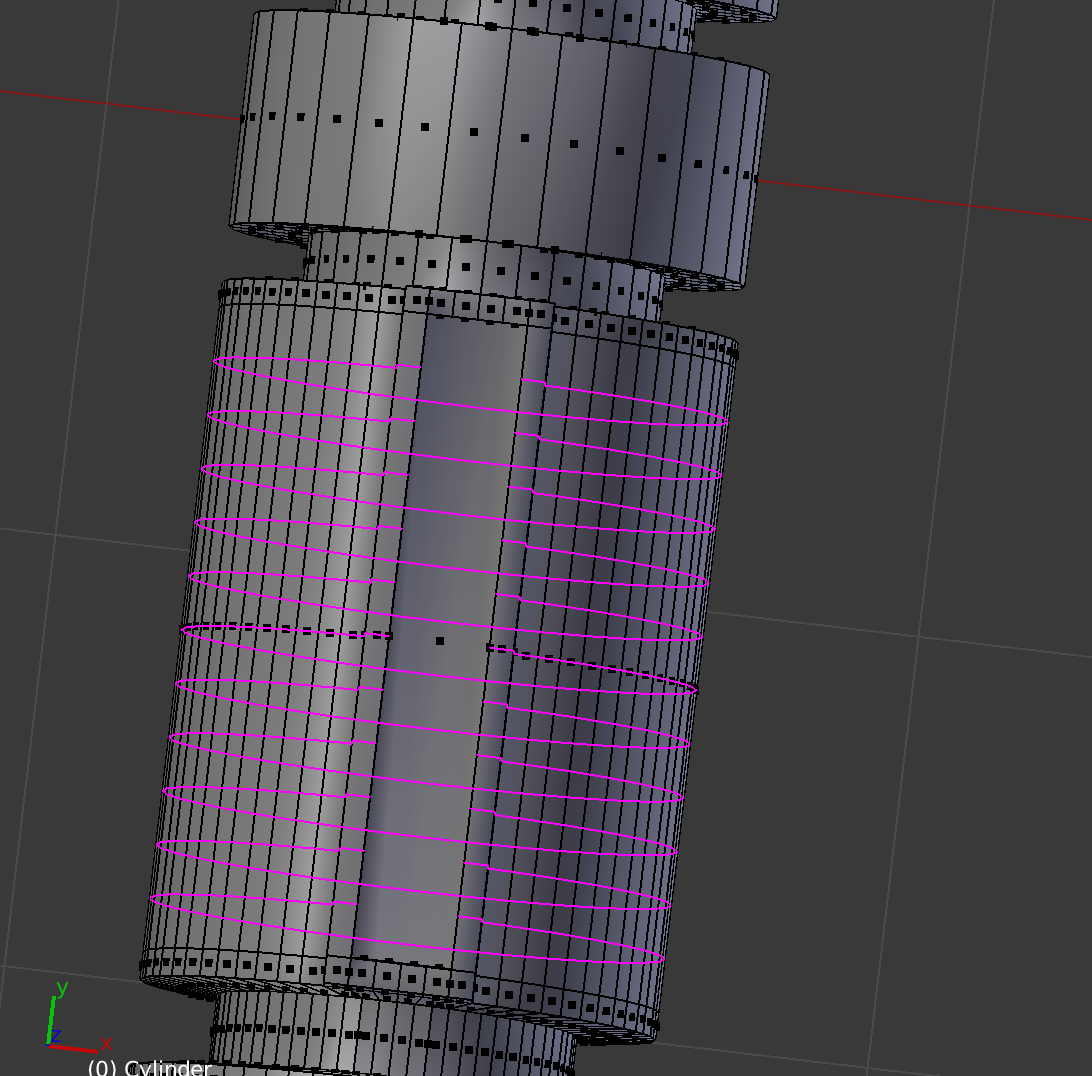
\includegraphics[scale=0.3]{./Capitulo1/Imagenes/10.png}
		\caption{Botones sable 2.}
	\label{10}
\end{figure} 


\begin{figure}
	\centering
		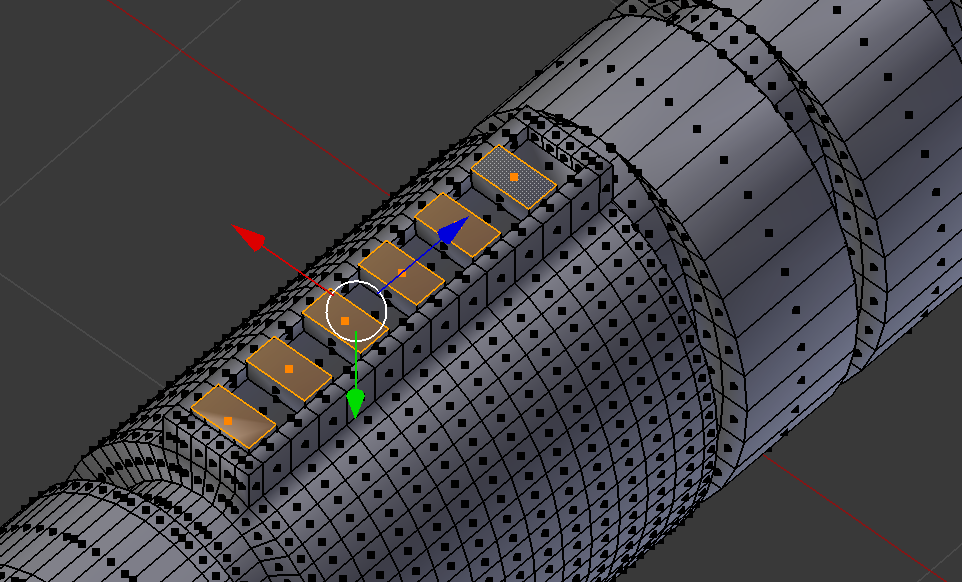
\includegraphics[scale=0.4]{./Capitulo1/Imagenes/11.png}
		\caption{Botones sable 3.}
	\label{11}
\end{figure} 


\begin{figure}
	\centering
		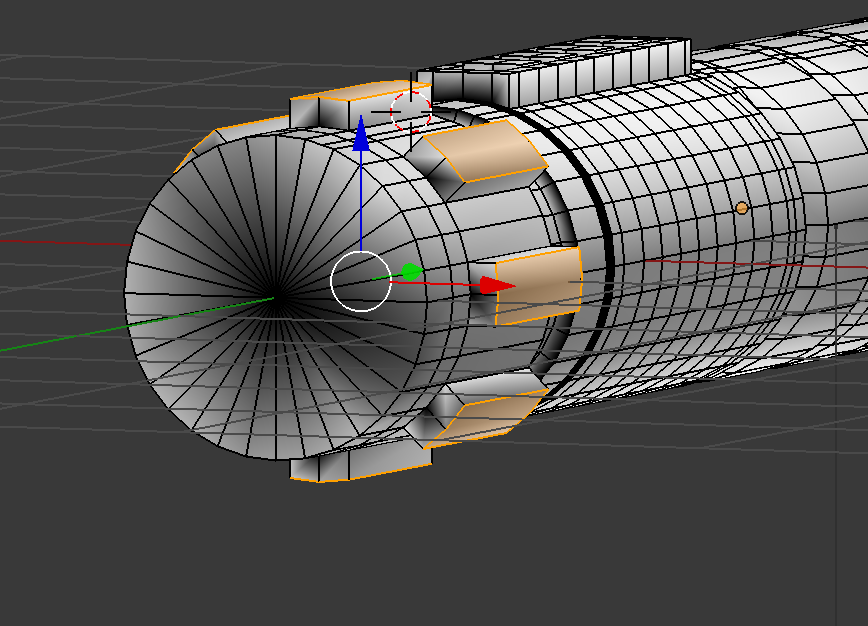
\includegraphics[scale=0.4]{./Capitulo1/Imagenes/13.png}
		\caption{Resaltes empu�adura.}
	\label{12}
\end{figure} 


En el segundo paso de adornado, a�adimos la argolla de sujecci�n, para ello a�adimos una curva Bezier que modelamos y a�adimos al sable donde corresponde. Para que sea mas realista, crearemos una cara donde los dos objetos interceden e introduciremos hacia dentro la misma para que la argolla parezca realmente introducida dentro del sable y no surgiendo de una de las caras de este como si nada. Este proceso lo podemos ver en las figuras \ref{13} y \ref{14}.


\begin{figure}
	\centering
		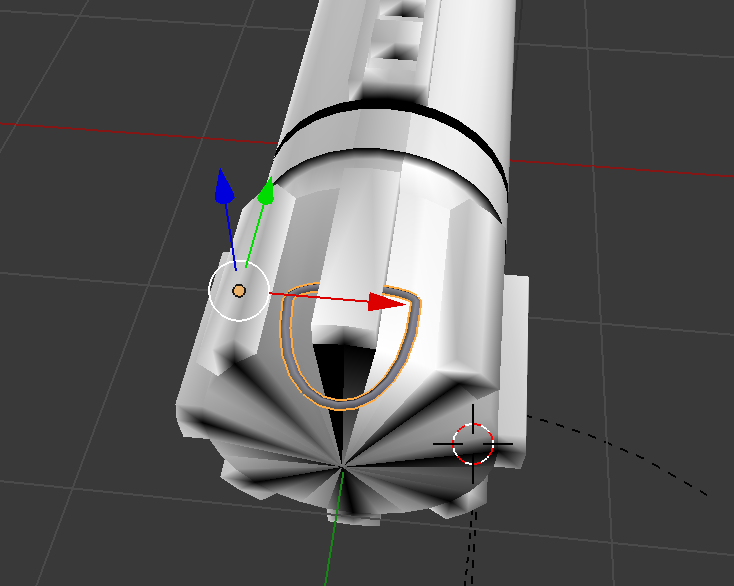
\includegraphics[scale=0.6]{./Capitulo1/Imagenes/14.png}
		\caption{Argolla 1.}
	\label{13}
\end{figure} 

\begin{figure}
	\centering
		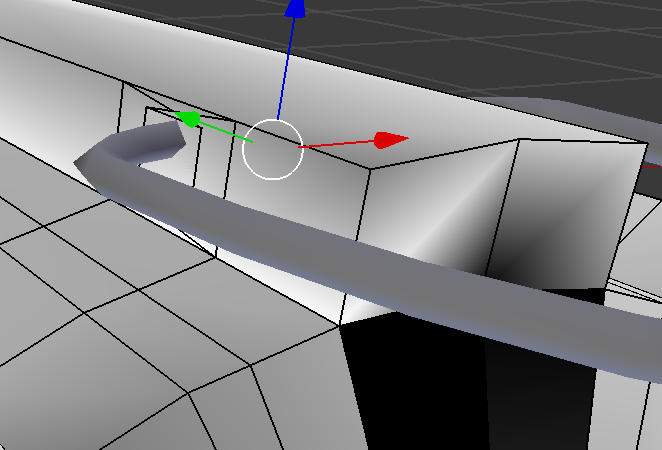
\includegraphics[scale=0.6]{./Capitulo1/Imagenes/15.png}
		\caption{Argolla 2.}
	\label{14}
\end{figure} 


El modelo final podemos verlo en la figura \ref{16}


\begin{figure}
	\centering
		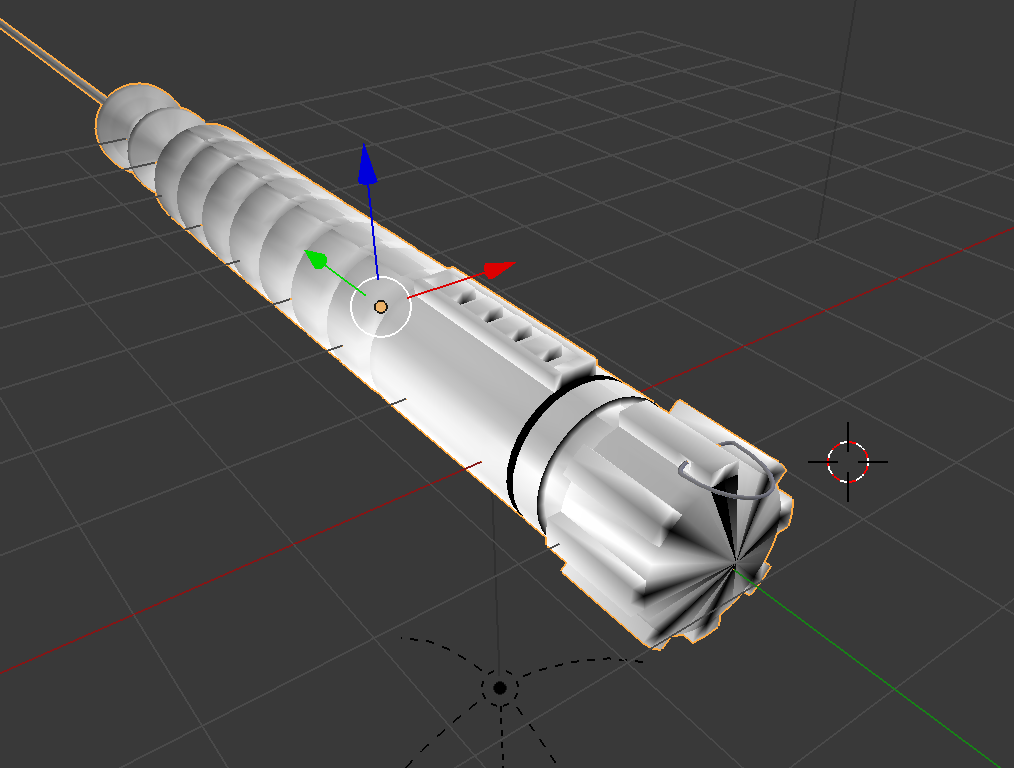
\includegraphics[scale=0.6]{./Capitulo1/Imagenes/16.png}
		\caption{Modelo final.}
	\label{16}
\end{figure} 


\clearpage
%---------------------------------------------------